\documentclass[useAMS,usenatbib]{mnras}

%_____GENERAL PACKAGES_____
\usepackage{amsmath}	%for \text{} in math mode
\usepackage{amssymb}	%for symbols

%_____FIGURES_____
\usepackage{graphicx}	%for including images
\usepackage{float}	%for [Hhtb] etc of figures
\usepackage{grffile}    %for using underscores in figure filenames
\usepackage{subcaption} %for having sub-captions in figures with multiple panels
\usepackage{placeins} %for \FloatBarrier, which forces all figures to be printed before continuing

%_____SYMBOLS_____
\usepackage{ mathrsfs } %for slanted letters in math mode

%_____FORMAT_____
\setcounter{secnumdepth}{2}	%depth of section numbering
\usepackage{hyperref} %ready-to-lick referencing

%_____MACROS______
\newcommand*\diff{\mathop{}\!\mathrm{d}}
\newcommand*\Diff[1]{\mathop{}\!\mathrm{d^#1}}
%\newcommand{\vect}[1]{\boldsymbol{#1}} % Uncomment for BOLD vectors.
\newcommand{\vect}[1]{\vec{#1}} % Uncomment for ARROW vectors.
\usepackage[usenames,dvipsnames]{xcolor}
\newcommand{\Wilma}[1]{\textcolor{Magenta}{#1}}

%%%%%%%%%%%%%%%%%%%%%%%%%%%%%%%%%%%%%%%%%%%%%%%%

\title[A spiral galaxy's mass distribution uncovered]{A spiral galaxy's mass distribution uncovered through lensing and dynamics}
\author[W. H. Trick, G. van de Ven and A. A. Dutton]{Wilma H. Trick$^{1}$\thanks{E-mail:
trick@mpia.de}, Glenn van de Ven$^{1}$ and Aaron A. Dutton$^{1}$\\
$^{1}$Max-Planck-Institute for Astronomy, K\"{o}nigstuhl 17, 69117 Heidelberg, Germany}
\begin{document}

\date{Accepted ???. Received ???; in original form ???}

\pagerange{\pageref{firstpage}--\pageref{lastpage}} \pubyear{2015}

\maketitle

\label{firstpage}

%--------------------------------------------
%Abstract
\begin{abstract}
We investigate the matter distribution of a spiral galaxy with counter-rotating stellar core, SDSS J1331+3628 (J1331), independently with gravitational lensing and dynamical modelling. By fitting a gravitational potential model to a quadruplet of lensing images around J1331's bulge, we tightly constrain the mass inside the Einstein radius $R_\text{ein}=(0.91\pm0.02)''(\simeq1.83\pm0.04~\text{kpc})$ to within 4\%: $M_\text{ein} = (7.8\pm0.3) \cdot 10^{10} M_\odot$. We model observed long-slit major axis stellar kinematics in J1331's central regions by finding Multi-Gaussian Expansion (MGE) models for the stellar and dark matter distribution that solve the axisymmetric Jeans equations. The lens and dynamical model are independently derived, but in very good agreement with each other around $\sim R_\text{ein}$. We find that J1331's center requires a steep total mass-to-light ratio gradient. A dynamical model including a NFW halo (with virial velocity $v_{200} \simeq 240 \pm 40~\text{km s}^{-1}$ and concentration of $c_{200} \simeq 8 \pm 2$) and moderate tangential velocity anisotropy ($\beta_z \simeq -0.4 \pm 0.1$) can reproduce the signatures of J1331's counter-rotating core and predict the stellar and gas rotation curve at larger radii. However, our models do not agree with the observed velocity dispersion at large radii. We speculate that the reason could be a non-trivial re-distribution of matter due to a possible merger event in J1331's recent past.
 %[Fertig.]
\end{abstract}
%--------------------------------------------

\begin{keywords}
gravitational lensing: strong -- stars: kinematics and dynamics -- galaxies: kinematics and dynamics -- galaxies: photometry -- galaxies: structure
\end{keywords}

%--------------------------------------------
%Introduction
\section{Introduction}

Gravitational lensing and dynamical modelling provide independent constraints on the mass distribution of galaxies. Combining them allows for valuable cross-checking opportunities to disentangle the stellar and dark matter (DM) content of galaxies.

Cosmological simulations suggest that cold DM forms cuspy halos following a Navarro-Frenk-White (NFW) profile \citep{NFW96}. However, the existence of central DM density cusps in massive galaxies depends strongly on the stellar mass-to-light ratio (e.g., \citealt{2011MNRAS.416..322D}) and DM dominated dwarf galaxies even favour DM halos with cores (e.g., \citealt{1994Natur.370..629M,2001ApJ...552L..23D}). This discrepancy, known as the core-cusp problem, might be resolved by galaxy formation processes such as mergers and outflows (e.g., \citealt{2001ApJ...560..636E,2012MNRAS.421.3464P}).

Determining the overall mass distribution in massive galaxies and separating the DM from the stellar mass components is therefore a crucial step in better understanding the structure and formation of galaxies and nature of DM.

Massive galaxies can act as gravitational lenses, deflect the light of background sources and give rise to multiple images. This strong gravitational lensing tightly constrains the projected total mass of the lens galaxy inside $\sim 1''$ (e.g., \citealt{2010ARA&A..48...87T}). 

The mass profile at larger galactocentric radii can be probed by gas rotation curves that directly measure the galaxy's circular velocity profile \Wilma{[TO DO: REF]}. However, due to its dissipative nature, gas motions are very sensitive to disturbances by e.g., spiral arms and bars \Wilma{[TO DO: REF]}. 

Because stars are dissipationless dynamical tracers and present almost everywhere in the galaxy, stellar dynamical modelling can complement mass constraints from lensing at small and gas motions at large radii. As stellar motions are complex---a bulk rotation around one principal axis combined with random motions in all coordinate directions---, full dynamical modelling of rotation, dispersion and velocity anisotropies is needed to deduce the matter distribution.

The Sloan WFC Edge-on Late-type Lens Survey (SWELLS, WFC = Wide field camera) \citep{SWELLSI,SWELLSII,SWELLSIII,SWELLSIV,SWELLSV,SWELLSVI} is dedicated to find and investigate spiral galaxies, which are (a) strong gravitational lenses and (b) seen almost edge-on, such that rotation curves can be easily measured. By combining lensing and dynamical modelling degeneracies inherent in both methods can be broken.

One of the SWELLS galaxies is the massive spiral SDSS J1331+3628, to which we refer as J1331 in the remainder of this work. It has bluish spiral arms and a large reddish bulge (see Figures \ref{fig:F450W} and \ref{fig:F814W}), which is superimposed by a quadruplet of extended bluish images approximately at a distance of $1''$ from the galaxy center (see Figure \ref{fig:lens_just_imgpos}). The lensed object might be a star-forming blob of a background galaxy. J1331 stands out of the SWELLS sample because of its large counter-rotating core (see Figure \ref{fig:kinematics}), which might be an indication that J1331 underwent a merger in its recent past.

\citet{SWELLSI} confirmed that J1331 was a strong gravitational lens, measured its apparent brightness and estimated the stellar masses of disk and bulge. The lensing properties of J1331 were first analysed by \citet{SWELLSIII}. \citet{SWELLSV} measured the gas and stellar kinematics along the major axis and deduced J1331's mass profile from the gas rotation curve at large radii and total mass inside the Einstein radius from gravitational lensing, focusing mostly on the outer regions of J1331.

The goal of this work is to complement the previous work on J1331 by an in-depth analysis of the matter distribution in J1331's inner regions. We use stellar dynamical modelling in addition to lensing constraints, similar to a study of the Einstein Cross by \citet{GlennEC}. We attempt to disentangle the stellar and DM components and test if employed axisymmetric Jeans models work also in the presence of a counter-rotating core. Ideally, this work on J1331 could also help understanding how mergers modify the mass distribution of a galaxy.

This paper is organized as follows: Section \ref{sec:data} summarizes the data, Section \ref{sec:Modelling} gives an overview of the modelling techniques used in this work, and Section \ref{sec:Results} presents our results on the surface photometry of J1331 using Multi-Gaussian expansions (Section \ref{sec:MGE_results}), constraints from lensing (Section \ref{sec:results_lensing}) and Jeans modelling based on the surface brightness only (Section \ref{sec:results_JAM_SB}) and including a NFW DM halo (Section \ref{sec:results_JAM_NFW}). Finally Section \ref{sec:Discussion} uses the result to discuss J1331's stellar mass-to-light ratio, possible merger history and starting points for future work.


%============================================================================


\begin{figure*}
\centering
\begin{subfigure}{.5\textwidth}
  \centering
  \includegraphics[width=.9\linewidth]{fig/first_glimpse_450.ps}
  \caption{J1331 in F450W}
  \label{fig:F450W}
\end{subfigure}%
\begin{subfigure}{.5\textwidth}
  \centering
  \includegraphics[width=.9\linewidth]{fig/first_glimpse_814.ps}
  \caption{J1331 in F814W}
  \label{fig:F814W}
\end{subfigure}
\begin{subfigure}{.5\textwidth}
  \centering
  \includegraphics[width=.9\linewidth]{fig/lens_imgpos.ps}
  \caption{The lensing images}
  \label{fig:lens_just_imgpos}
\end{subfigure}%
\begin{subfigure}{.5\textwidth}
  \centering
  \includegraphics[width=.9\linewidth]{fig/stellar_kinematics_data.ps}
  \caption{Stellar Kinematics by \citet{SWELLSV}}
  \label{fig:kinematics}
\end{subfigure}
\caption{Hubble Space telescope (HST) images and stellar kinematics of the galaxy SDSS J1331+3628 (J1331), which has a large counter-rotating core and whose bulge acts as a strong lens for a bluish background source. \emph{Panel (a) and (b):} HST/WFPC2/WFC3 images of J1331 by \citet{SWELLSI} in two filters, F450W in panel (a) and F814W in panel (b). The black solid line in panel (b) shows the orientation of the major-axis. Its length is $10''$ and it indicates approximately where we carry out the dynamical modelling. \emph{Panel (c):} Lensing images in the central region of J1331.  An IRAF \emph{ellipse} fit to the F450W surface brightness in panel (a) was subtracted from the image. The (smoothed) residuals within the white square in panel (a) are shown in panel (c). (The four bright blobs (A,B,C and D), that become visible, are arranged in a typical strong lensing configuration around the center of the galaxy (G). The configuration of the two additional blobs, that lie approximately on a line with A, B and G, does not suggest that they form a lensing doublet. They might be star forming regions of a background galaxy.) \emph{Panel (d):} Stellar Kinematics along the galaxy's major axis as measured by \citet{SWELLSV}, line-of-sight rotation velocity $v_\text{rot}$, line-of-sight velocity dispersion $\sigma$ and the rms-velocity $v_\text{rms} = \sqrt{v_\text{rot}^2 + \sigma^2}$. The dotted line in panel (b) indicates the galaxy's effective half-light radius (in the F814W filter), $R_\text{eff} = 2.6" = 5.2~\text{kpc}$. The $v_\text{rot}$ curve reveals that J1331 has a counter-rotating core within $R_\text{eff}$. \Wilma{[TO DO: No dotted line]}}
\label{fig:specialJ1331}
\end{figure*} %[Fertig gekuerzt. Es fehlen noch 2 Referenzen.]
%--------------------------------------------

%------------------------
\section{Data} \label{sec:data}

\paragraph{Redshift and position.} J1331 is located at right ascension = 202.91800$^\circ$ and a declination = 36.46999$^\circ$ (epoch J2000). \citet{SWELLSI} found from SDSS spectra that J1331 has two redshifts inside $1''$: J1331 itself has $z_d = 0.113$ and $z_s = 0.254$ is the redshift of the lensed background source \citep{SWELLSIII}. According to the WMAP5 cosmology \citep{WMAP5cosm}, J1331 has an angular diameter distance of 414 Mpc, which translates into a transverse scaling of $1'' \hat{=} 2.01~\text{kpc}$.

\paragraph{HST imaging.} We use HST imaging of J1331 by \citet{SWELLSI}. They performed high resolution imaging with the Hubble Space Telescope's (HST) Wide-Field Planetary Camera 2 (WFPC2) and its WF3 CCD chip. The images are a combination of four exposures with each an exposure time of $400~\text{sec}$ and were drizzled to a pixel scale of 1 pixel = $0.05''$. In particular, we use the images in the filters F450W, to identify the positions of the bluish lensing images, and F814W (I-band) to create a surface brightness MGE model of the reddish bulge.

\paragraph{Stellar kinematics.} For the dynamical modelling we use the stellar kinematics for J1331 measured by \citet{SWELLSV}. They obtained long-slit spectra along J1331's major-axis with the Low Resolution Imaging Spectrograph (LRIS) on the Keck I 10m telescope. The width of the slot was $1''$ and the seeing conditions had a FWHM of $\sim 1.1''$. Spectra for spatial bins of different widths along the major axis were extracted. They measured line-of-sight stellar rotation velocities ($v_\text{rot}$) and stellar velocity dispersion ($\sigma$) by fitting Gaussian line profiles to emission \Wilma{[TO DO: Check if really emission lines or, more likely, absorption lines]} lines in these spectra \Wilma{[TO DO: Find out which lines]}. Gas kinematics were extracted from fits to H$\alpha$ and NII lines, as tracers for ionized gas.
\\The stellar kinematics, $v_\text{rot}$, $\sigma$ and $v_\text{rms}^2=v_\text{rot}^2 + \sigma^2$ are shown in Figure \ref{fig:kinematics}. The rotation curve reveals a counter-rotating core within $2''\simeq$ 4 kpc. Outside of $\sim 3.5''$ there is a steep drop in the dispersion, which is expected at the boundary between the pressure supported bulge and the rotationally supported disk, which appears around this radius in the F450W filter in Figure \ref{fig:F450W}. However, in the brighter F814W filter in Figure \ref{fig:F814W}  the large reddish bulge extends out to $\sim5''$. 
\\Inside of $\sim 4''$, the data appears to be symmetric, outside of this the assumption of axisymmetry seems not to be valid anymore, considering the data. We add $-2.3~\text{km s}^{-1}$ to the $v_\text{rot}$ to ensure $v_\text{rot}(R'=0) \sim 0$ as a possible correction term for a misjudgement of the systemic velocity. We also symmetrize the data within $4''$ and asign a minimum error of $\delta v_\text{rms} > 5~\text{km s}^{-1}$ to the $v_\text{rms}$ data. In the JAM modelling, which is based on the assumption of axisymmetry, only stellar kinematics with $R'  \lesssim 2.5''$ or $R' \lesssim 4''$ are used. Another reason to restrict to modelling on the bulge region is that our MGE in Table \ref{tab:MGEF814W} is only a good representation of J1331's F814W light distribution inside $\sim 5''$.

 \Wilma{[TO DO: Maybe mention the following details better in the data section.... "Sufficiently inclined galaxies were picked by eye. Follow-up high resolution imaging with the Hubble Space Telescope's (HST) Wide-Field Planetary Camera 2 (WFPC2) was performed to confirm their lensing status \citep{SWELLSI}."]} %[Not done yet]
%------------------------

%------------------------
\section{Modelling} \label{sec:Modelling}
\input{docs/model_MGE_v3.02} %[Fertig]
\subsection{Strong gravitational lens model} \label{sec:lensing_theo}

\paragraph{Lensing formalism.} A gravitational lens is a mass distribution, whose gravitational potential $\Phi$ acts as a lens for light coming from a source positioned somewhere on a plane behind the lens. The angular diameter distance from the observer to the lens is $D_d$, to the source plane $D_s$, and the distance between the lens and source plane is $D_{ds}$. The deflection potential of the lens is its potential, projected along the line of sight $z$ and rescaled to
\begin{equation}
\psi(\vect{\theta}) := \frac{D_{ds}}{D_d D_s} \frac{2}{c^2} \int \Phi(\vect{r}=D_d \vect{\theta},z) {\ \mathrm d} z, \label{eq:psidef}
\end{equation}
where $\vect{\theta}$ is a 2-dimensional vector on the plane of the sky. The light from the source at $\vect{\beta} = (\xi,\eta)$\footnote{$\xi$ and $\eta$ are cartesian coordinates on the plane of the sky.} is deflected according to the lens equation
\begin{equation}
\vect{\beta} = \vect{\theta}_i - \left.\vect{\nabla}_\theta \psi(\vect{\theta})\right|_{\vect{\theta}_i} \label{eq:lenseqpot}
\end{equation}
into an image $\vect{\theta}_i = (x_i,y_i)$. The gradient of the deflection potential $\vect{\nabla}_\theta \psi(\vect{\theta})$ is equal to the angle by which the light is deflected multiplied by $D_{ds}/D_{s}$.

The total time delay of an deflected light path through $\vect{\theta}$ with respect to the unperturbed light path is given by 
\begin{equation}
\Delta t(\vect{\theta}) = \frac{(1+z_d)}{c} \frac{D_d D_s}{D_{ds}} \left[ \frac 12 (\vect{\theta} - \vect{\beta})^2 - \psi(\vect{\theta})\right] \label{eq:timedelay}
\end{equation}
\citep{BartGravLens}. According to Fermat's principle the image positions will be observed at the extrema of $\Delta t(\vect{\theta})$.

The inverse magnification tensor
\begin{equation}
\mathscr{M}^{-1} \equiv \frac{\partial \vect{\beta}}{\partial \vect{\theta}} \overset{(\ref{eq:lenseqpot})}{=} \left(\delta_{ij} - \frac{\partial^2 \psi}{\partial \theta_i \partial \theta_j} \right)\label{eq:magnificationtensor}
\end{equation}
describes how the source position changes with image position. It also describes the distortion of the image shape for an extended source and its magnification due to lensing according to
$$\mu \equiv \frac{\text{image area}}{\text{source area}} = \det \mathscr{M}.$$
Lines in the image plane for which the magnification becomes infinite, i.e., $\det \mathscr{M}^{-1} = 0$, are called critical curves. The corresponding lines in the source plane are called caustics. The position of the source with respect to the caustic detemines the number of images and their configuration and shape with respect to each other.

The Einstein mass $M_\text{ein}$ and Einstein radius $R_\text{ein}$ are defined via the relation
\begin{equation*}
M_\text{ein} \equiv M_\text{proj}(<R_\text{ein}) \overset{!}{=} \pi \Sigma_\text{crit} R_\text{ein}^2,
\end{equation*}
where $\Sigma_\text{crit} \equiv \frac{c^2}{4\pi G} \frac{D_s}{D_d D_{ds}}$ is the critical density and $M_\text{proj}(<R_\text{ein})$ is the mass projected along the line-of-sight within $R_\text{ein}$. $M_\text{ein}$ is similar to the projected mass within the critical curve $M_\text{crit}$.

\paragraph{Lens model.} Following \citet{EvansWitt} we assume a scale-free model
\begin{equation}
\psi(R',\theta') = R^{'\alpha} F(\theta') \label{eq:scalefreemodel}
\end{equation}
for the lensing potential, consisting of an angular part $F(\theta')$ and a power-law radial part, with $(R',\theta')$ being polar coordinates on the plane of the sky. The case $\alpha = 1$ corresponds to a flat rotation curve. We expand $F(\theta')$ into a Fourier series,
\begin{equation}
F(\theta') = \frac{a_0}{2} + \sum_{k=1}^{\infty} \left(a_k \cos(k\theta') + b_k \sin (k\theta') \right). \label{eq:Fourieransatz}
\end{equation}
For this scale-free lens model the lens equation \eqref{eq:lenseqpot} becomes
\begin{equation}
\begin{pmatrix} \xi \\ \eta \end{pmatrix} = \begin{pmatrix} R'_i \cos \theta'_i - R_i^{'\alpha-1} \left(\alpha \cos \theta'_i F(\theta'_i) - \sin \theta'_i F'(\theta'_i) \right) \\ R'_i \sin \theta'_i - R_i^{'\alpha-1} \left(\alpha \sin \theta'_i F(\theta'_i + \cos \theta'_i F'(\theta'_i) \right)\end{pmatrix}\label{eq:Fourierlenseq}
\end{equation}
\citep{EvansWitt}, where $F'(\theta') \equiv \partial F(\theta') / \partial \theta'$. When we fix the slope $\alpha$, then the lens equation is a purely linear problem and can be solved numerically for the source position $(\xi,\eta)$ and the Fourier parameters $(a_k,b_k)$ given one observed image at position $(x_i=R'_i \cos \theta'_i,y_i=R'_i \sin \theta'_i)$. 

\paragraph{Model fitting.} The free parameters of the lens model are: the source position $(\xi,\eta)$, the radial slope $\alpha$ and Fourier parameters $(a_k,b_k)$ of the lens mass distribution in Equations \eqref{eq:scalefreemodel} and \eqref{eq:Fourieransatz}. We want to minimize the distance between the observed image positions, $\vect{\theta}_{oi}$, and those predicted by the lensing model, $\vect{\theta}_{pi}$. To avoid having to solve the lens equation \eqref{eq:Fourierlenseq} for $\vect{\theta}_{pi}$, we follow \citet{1991ApJ...373..354K} and cast the calculation back to the source plane using the magnification tensor in Equation \eqref{eq:magnificationtensor} to approximate $\vect{\theta} \simeq (\partial \vect{\theta} / \partial \vect{\beta}) \vect{\beta} = \mathscr{M} \vect{\beta} $. The best fit lens model is then the one that minimizes
\begin{eqnarray*}
\chi^2_\text{lens} &=& \sum_{i} \left|\left( \begin{matrix} \frac{1}{\Delta_x} & 0\\0 & \frac{1}{\Delta_y}\end{matrix}\right) \left( \vect{\theta}_{pi} - \vect{\theta}_{oi} \right)\right|^2\\
&\simeq& \sum_{i} \left|\left( \begin{matrix} \frac{1}{\Delta_x} & 0\\0 & \frac{1}{\Delta_y}\end{matrix}\right)  \left.\mathscr{M}\right|_{\vect{\theta}=\vect{\theta}_{oi}} \left( \begin{matrix} \xi - \tilde{\xi}_i \\ \eta - \tilde{\eta}_i \end{matrix} \right) \right|^2,
\end{eqnarray*}
where $(\Delta_x,\Delta_y)$ are the measurement errors of the image positions $\vect{\theta}_{oi}$. $\left.\mathscr{M}\right|_{\vect{\theta}=\vect{\theta}_{oi}}$ is the magnification tensor and $(\tilde{\xi}_i,\tilde{\eta}_i)$ the source position according to the lens equation, both evaluated at the position of the $i$-th lensing image, $\vect{\theta}_{oi}$. Following \citet{GlennEC} we add a term
\begin{equation*}
\chi^2_\text{shape} = \lambda \sum_{k \geq 3} \frac{\left(a_k^2 +b_k^2 \right)}{a_0^2} 
\end{equation*}
which forces the shape of the mass distribution to be close to an ellipse. The total $\chi^2$ to minimize is therefore
\begin{equation*}
\chi^2 = \chi^2_\text{lens} + \chi^2_\text{shape}
\end{equation*}
We set $a_1 = b_1 = 0$, which corresponds to the choice of origin; in this case the center of the galaxy.

To be able to constrain the slope $\alpha$, we would need flux ratios for the images as in \citet{GlennEC}. But the extended quality of the images, possible dust obscuration and surface brightness fluctuations due to microlensing events, as well as the uncertainty in surface brightness subtraction, make flux determination too unreliable and we do not include them in the fitting. %[Fertig]
\input{docs/model_JAM_v3.02} %[Fertig - wenn auch nicht so toll.]
%------------------------

%------------------------
\section{Results} \label{sec:Results}
%============================================================================
\begin{table}
\centering
\caption{Galaxy parameters of J1331.}
\begin{tabular}{lllr}
\hline
redshift \citep{SWELLSIII}                 & $z_d$ & $0.113$ \\
angular diameter distance & $D_d$ [Mpc] & $414$ \\
scaling                   & 1 kpc / 1$''$ & $2.006$ \\
position angle from North          & $\phi$ [degrees] & $42.90^\circ$\\
average axis ratio & $q'$ & $0.598$\\
average ellipticity & $\epsilon = 1 - q'$ & $0.402$ \\
estimated inclination & $i$ [degrees] & $70^\circ$\\
apparent I-band magnitude & $m_\text{I}$ [mag] & $15.77$ \\
total I-band luminosity & $L_\text{I,tot}$ [$10^{10} L_\odot$] & $5.6$ \\
effective half-light radius & $R_\text{eff}$ [$''$] & $2.6$ \\
& $R_\text{eff}$ [pc]& 5.2 & \\
\hline
\end{tabular}
\label{tab:galaxyparameters}
\end{table}
%============================================================================

\subsection{Surface photometry for J1331 with MGEs} \label{sec:MGE_results}

In this section we construct a model for the J1331's intrinsic light distribution in terms of MGEs (see Section \ref{sec:MGE_theo}). We use the HST image in the F814W (I-band) filter (Figure \ref{fig:F814W}) because J1331's central stellar component appears at longer wavelengths (i) smoother and more extended than in the F450W filter (Figure \ref{fig:F450W}), as it is less sensitive to young clumpy star-forming regions, (ii) much brighter than the bluish lensing images, and (iii) the imaging is less prone to extinction.

\paragraph{PSF for the HST/F814W filter.} The one-dimensional MGE in Equation \eqref{eq:PSFgeneral} is fitted to the radial profile of a synthetic image of the HST/F814W filter PSF, ignoring diffraction spikes and using the code by \citet{Cap02}. The MGE parameters of the normalized PSF model are given in Table \ref{tab:PSFMGEF814W}.

%============================================================================
\begin{table}
\centering
\caption{F814W PSF MGE: Parameters of the circular four-Gaussian MGE in Equation \eqref{eq:PSFgeneral} fitted to the radial profile of the synthetic HST/F814W PSF image.}
\begin{tabular}{ccc}
\hline
$j$ & $G_j$ & $\delta_j$ [$''$] \\\hline
1 & 0.184 & 0.038\\
2 & 0.485 & 0.085\\
3 & 0.222 & 0.169\\
4 & 0.109 & 0.487\\\hline
\end{tabular}
\label{tab:PSFMGEF814W}
\end{table}
%============================================================================

\paragraph{MGE for the inner regions.} We fit a MGE to J1331's smooth central region within $\sim 5''$ from the HST/WFPC2/WF3/F814W image (Figure \ref{fig:F814W}). Bright objects close to the bulge (blobs possibly belonging to the background galaxy and parts of the foreground spiral arm) were masked during the fit. J1331's galaxy center, position angle (with respect to North through East) and average apparent ellipticity (see Table \ref{tab:galaxyparameters}) are found from the images weighted first and second moment. The MGE fit splits the image in annuli with the given ellipticity and position angle and sectors of $5^\circ$ width and fits an 5-Gaussian MGE of the form in Equation \eqref{eq:MGEgeneral} convolved with the PSF MGE in Table \ref{tab:PSFMGEF814W} to it. The best fit MGE (PSF convolved) is compared to the data in Figure \ref{fig:MGEinnerRegions} and the corresponding parameters of the intrinsic surface brightness distribution are given in Table \ref{tab:MGEF814W}. The fit is a very good representation of the light distribution in the inner $5''$, but underestimates the light distribution outward.

\paragraph{MGE for the outer regions.} To get a handle on the light distribution also in the outer parts of J1331, where spiral arms dominate, we first fit a IRAF \citep{1993ASPC...52..173T} \emph{ellipse} model to the F814W image (masking the brightest blobs in the spiral arms and outer regions). Only then we fit a 7-Gaussian MGE to the smooth ellipse model. The MGE does not perfectly reproduce the flatness of the ellipse model at every radius (see Figure \ref{fig:MGEouterRegions}), but considering the spiral arm dominated outer regions of J1331, it is good enough for an approximate handling of the overall light distribution.

\paragraph{Transformation into physical units.} To transform the MGE in units of counts into physical units, we apply a simplified version of the procedure described in \citet{Holtzman}.

%============================================================================
\begin{figure*}
\centering
\begin{subfigure}{.5\textwidth}
  \centering
  \includegraphics[width=.8\columnwidth]{fig/1331F814Wsci_MGE_M.ps}
  \caption{MGE for J1331's inner regions.}
 \label{fig:MGEinnerRegions}
\end{subfigure}%
\begin{subfigure}{.5\textwidth}
  \centering
  \includegraphics[width=.8\columnwidth]{fig/1331F814W_MGE_disk_L.ps}
  \caption{MGE and IRAF \emph{ellipse} model for J1331's outer regions.}
 \label{fig:MGEouterRegions}
\end{subfigure}%
\caption{MGEs for J1331's surface brightness distribution. Comparison of contours with constant F814W surface brightness (orange lines) with the corresponding iso-brightness contours of the best fit MGE, convolved with the PSF in Table \ref{tab:MGEF814W}, (grey lines). The black line has a length of $10''$ and its orientation corresponds to the galaxy's position angle as found in Table \ref{tab:galaxyparameters}. For comparison the Einstein radius as found in Table \ref{tab:bestfitlensmodel}  is indicated as red dashed circle. \emph{Panel (a):} Central regions of J1331. The MGE model is a good representation of the galaxy's light distribution along the major axis within $\sim 5''$. Its parameters are given in Table \ref{tab:MGEF814W}. This MGE is used as model for the stellar tracer distribution in the dynamical Jeans modelling in Sections \ref{sec:results_JAM_SB} and \ref{sec:results_JAM_NFW}. \emph{Panel (b):} Outer regions of J1331. The orange lines indicate here contours of a smooth IRAF \emph{ellipse} fit to J1331 in the F814W filter; the grey lines are the corresponding best fit MGE. This MGE is not used for dynamical modelling, because the dynamics in the outer regions are strongly affected by non-axisymmetries (e.g., spiral arms). We use it, however, to estimate the galaxy's total luminosity and effective radius, and to get a prediction for the dynamics of the outer regions.}
\end{figure*}
%============================================================================

%============================================================================
\begin{table*}
\centering
\caption{Parameters of the best fit MGE to the F814W surface brightness of J1331 in Figure \ref{fig:MGEinnerRegions}. The fit is best inside an radius of $5''$. The position angle is given in Table \ref{tab:galaxyparameters}. This MGE is used in the dynamical modelling in Sections \ref{sec:results_JAM_SB} and \ref{sec:results_JAM_NFW}. The first column gives for each Gaussian the total F814W luminosity in Equation \eqref{eq:centralItotalL} in units of counts. The second column is the corresponding I-band peak surface brightness in Equation \eqref{eq:MGEgeneral} in units of a luminosity surface density. The third and fourth column give the dispersion and the last column the axis ratio of the Gaussian in Equation \eqref{eq:MGEgeneral}.}
\begin{tabular}{cccccc}
\hline
 & total luminosity  & surface density & \multicolumn{2}{c}{Gaussian dispersion} & axis ratio\\
$i$  & $L_i$ [counts] & $I_{0,i}$ [$L_\odot$/pc$^2$] & $\sigma_i$ [$''$] & $\sigma_i$ [kpc] & $q'_i$\\\hline
1  &     9425.96 &      20768.  &  0.051   & 0.103  & 1.00\\
2  &    13173.0 &        3161.2 &  0.178   & 0.358  & 0.76\\
3  &    40235.0 &        1588.2 &  0.503   & 1.008  & 0.58\\
4  &    67755.2 &         502.25&  1.180   & 2.368  & 0.56\\
5  &    203677. &         136.51&  3.891   & 7.805  & 0.57\\\hline
\end{tabular}
\label{tab:MGEF814W}
\end{table*}
%============================================================================

The scaling of the drizzled HST/WFC3 images is  $S \equiv 0.05''/\text{pixel width}$ and the total exposure time $T = 1600$ sec. Each Gaussian in the MGE has a total F814W luminosity $L_i$ (in counts) and a central surface brightness (in counts per pixel) of
\begin{equation*}
C_{0,i}\text{[counts/pixel]} = \frac{L_i[\text{counts}]}{2\pi \sigma[\text{pixel}]^2 q}.
\end{equation*}
This is then transformed into an I-band surface brightness (in $\text{mag}\times(1'')^{-2}$) via
\begin{equation}
\mu_{I,0,i} \simeq -2.5 \log_{10}\left( \frac{C_{0,i}\text{[counts/pixel]}}{T[\text{sec}] \cdot S[''/\text{pixel width}]^2}\right) + Z + C + A_I, \label{eq:muI_}
\end{equation}
where $Z\simeq21.62~\text{mag}$ is a the zero-point from \citet{Holtzman}, updated according to \citet{Dolphin,DolphinNew}, for the photometric system of the HST/WFPC2 camera and the F814W filter, plus a correction for the difference in gain between calibration and observation. $C= 0.1~\text{mag}$ corrects for the finite aperture of the WFPC2; and $A_I =0.015~\text{mag}$ is the extinction in the (Landolt) I-band towards J1331, according to the NASA/IPAC Extragalactic Database (NED)\footnote{The NASA/IPAC Extragalactic Database (NED, \url{https://ned.ipac.caltech.edu/}) is operated by the Jet Propulsion Laboratory, California Institute of Technology, under contract with the National Aeronautics and Space Administration. The data for J1331 (SDSS J133140.33+362811.9) was retrieved in October 2013.}. The color-dependent correction between the F814W filter and the I-band of the UBVRI photometric system is  small \citep{Holtzman} and we neglect it therefore. The last step is to transform the surface brightness $\mu_{I,0,i}$ (in mag) to the I-band surface density $I_{0,i}$ (in $L_\odot$/pc$^2$) of the Gaussian, i.e.,
\begin{eqnarray*}
I_{0,i}[L_\odot \text{pc}^{-2}] = \left( 64800/\pi\right)^2 \left(1+z_d \right)^4 10^{0.4\left(M_{\odot,I}-\mu_{I,0,i} \right)},
\end{eqnarray*}
where the term with $z_d$ accounts for redshift dimming and $M_{\odot,I}=4.08~\text{mag}$ is the Sun's absolute I-band magnitude \citep{1998gaas.book.....B}. The luminosity $L_i$[counts] and the corresponding surface brightness density $I_{0,i} [L_\odot \text{pc}^{-2}]$ of each Gaussian are given in Table \ref{fig:MGEinnerRegions}.

\paragraph{Inclination.} To estimate the inclination of J1331 with respect to the observer, we use the observed axis ratio of the flattest ellipse in the IRAF \emph{ellipse} model for J1331, which is $q'=0.42$. This is similar to the disk axis ratio of $q' = 0.40$ found by \citet{SWELLSI}. If a typical thickness of an oblate disk is around $q_0 \sim 0.2$ \citep{1958MeLu2.136....1H}, the inclination follows from 
\begin{equation*}
\cos^2 i = \frac{q'^2 - q_0^2}{1 - q_0^2}
\end{equation*}
and a correction of $+3^\circ$ \citep{1988ngc..book.....T}. Our estimate for the inclination is therefore $i \approx 70^\circ$. Given this inclination, the 2D MGE models can be deprojected into three dimensions (see Section \ref{sec:MGE_theo}).

\paragraph{Total luminosity and effective radius.} J1331's total I-band luminosity is determined by summing up the luminosity contributions of all the MGE Gaussians for the outer regions (shown as grey lines in Figure \ref{fig:MGEouterRegions}). We find $L_\text{I,tot} \simeq 5.6 \cdot 10^{10} ~L_\odot$. This corresponds to an apparent magnitude of $m_I = 15.77~\text{mag}$. We determine the circularized effective radius $R_\text{eff}$ of J1331 from the definition $L(<R_\text{eff}) \equiv \frac 12 L_\text{tot}$ and the growth curve $L(<R')$ from the MGE model of the outer regions, where $R'$ is the projected radius on the sky. We find the effective radius to be $R_\text{eff} \simeq 2.6'' \hat{=} 5.2 \text{ kpc}$.  All values are summarized in Table \ref{tab:galaxyparameters}.


 %[Text bin ich durchgegangen. Allerdings muessen Captions noch ueberarbeitet werden.]
\subsection{Mass distribution from lensing} \label{sec:results_lensing}

\paragraph{Image positions.} We determine the positions of the lensing images by first subtracting a smooth model for the galaxy's surface brightness from the original image. As models we use MGE fits and IRAF \emph{ellipse} fits  (see Sections \ref{sec:MGE_theo} and \ref{sec:MGE_results})  to the galaxy in each the F450W and F814W filter. (For example the MGE we use for F814W is the MGE given in Table \ref{tab:MGEF814W} convolved with the PSF in Table \ref{tab:PSFMGEF814W}.) The lensing images become then visible in the residuals (see Figure \ref{fig:lens_just_imgpos}), in which we smooth out noise smaller than the PSF. Because the lensing images are extended, we use the position of the brightest pixel in each of the images. We also use the F450W-MGE subtracted residuals from \citet{SWELLSIII}. The lensing positions as determined from the latter are given in Table \ref{tab:lenspos}. The scatter of lensing positions as determined from subtracting different surface brightness models from the galaxy in different filters gives an error of $\pm 1$ pixel on the image positions. We find slightly different positions for the peak of the surface brightness in the different filters and apply correspondingly an error of one diagonal pixel to the brightness peak in the F450W image which we use as center of the galaxy.
\\Eight image position coordinates allow us to fit a lens mass model with only $<8$ free parameters. We therefore do not fit Fourier components $(a_k,b_k)$ with $k > 3$.
\\Even though the constraints from the image positions on $\alpha$ is very weak, we were however able to show that the image positions in Table \ref{tab:lenspos} are consistent with a model with flat rotation curve. In the following we therefore set $\alpha=1$.

\begin{table}
\centering
\begin{minipage}{70mm}
\begin{tabular}{r|rrrr|c}
\hline
  & A & B & C & D & G\\\hline
$x_i$ [pixel] & 12.1 & -8.5 & 21.7 & -3.3 & 0.5 $\pm \sqrt{2}$ \\
$y_i$ [pixel] & 16.6 & -10.4 & -0.5 & 19.2 & 0.5 $\pm \sqrt{2}$ \\
\hline
\end{tabular}
\caption{Positions of the lensing images (A-D) and the galaxy center (G) in Figure \ref{fig:lens_just_imgpos}. The image positions were determined from the lens subtracted image for J1331 in Figure 4 of \citet{SWELLSIII}, rotated to the $(x,y)$ coordinate system in Figure \ref{fig:lens_just_imgpos}. The pixel scale is 1 pixel = $0.05''$ and the error of each image position is $\pm$ 1 pixel.}
\label{tab:lenspos}
\end{minipage}
\end{table}


\paragraph{Best fit lens model.} The best fit lens model for the image positions in Table \ref{tab:lenspos} is given in the first column of Table \ref{tab:bestfitlensmodel}. Figure \ref{fig:lensbestfiteinsteincurves} shows the corresponding critical curve, caustic and Einstein radius, and the best fit source position. In this case, where $\alpha=1$, the critical curve is also an equidensity contour of the galaxy model \citep{EvansWitt}, which appears to have an elliptical mass distribution. This cricital curve is called \emph{tangential}, because of the tangential orientation of the images close to it. The source is located close to a cusp of the diamond-shaped caustic: a lensing configuration for which we indeed expect four images. This is a good indication that indeed all four images are indeed lensing images of the same object. Figure \ref{fig:lensbestfittimedelay} overplots the smoothed residuals from the F450W image subtracted by the IRAF \emph{ellipse} fit to the surface brightness with the contours of the best fit model's time delay surface. This demonstrates that, although we did not include any information about the shape of the lensing images in the fit, it is consistent with the predicted distortion for an extended source by the best fit lens model.
\\To estimate how the uncertainties in the determination of the image positions and galaxy center affect the results, we Monte Carlo sample random positions from a two-dimensional Normal distribution centered at the positions in Table \ref{tab:lenspos} and a standard deviation corresponding to the measurement error. A Gaussian fit to the resulting distributions of best fit values leads to the constraints on the shape parameters and Einstein quantities in the second column in Table \ref{tab:bestfitlensmodel}. We therefore constrain the Einstein radius to within 2\%, $R_\text{ein} = (0.91 \pm 0.02)''$ and the projected mass within the critical curve with a relative error of 4\%, $M_\text{crit} =(7.9\pm0.3)\cdot 10^{10} M_\odot$. Our measurement of $R_\text{ein}$ is consistent with that from \citet{SWELLSIII}, $R_\text{ein,SWELLS} = (0.96 \pm 0.04)''$ (which used a singular isothermal ellipsoid as lens mass model and the intermediate-axis convention of the critical curve as the Einstein radius). The relative difference between our critical mass and that of \citet{SWELLSIII}, $M_\text{crit,SWELLS} =(8.86\pm0.61)\cdot 10^{10} M_\odot$, is 13\%.

%========================================================================================

\begin{table*}
\centering
\caption{Best fit lens model found from the peak image positions in Table \ref{tab:lenspos} (first column) following the procedure described in Section \ref{sec:lensing_theo} and assuming a flat rotation curve ($\alpha = 1$). The second column gives the corresponding best fit mean and standard deviation derived from Monte Carlo sampling of the Gaussian uncertainties around the image positions (column 2).}
\begin{tabular}{llrrclr}
\hline
 &  & \multicolumn{1}{c}{lens model for} &\multicolumn{4}{c}{lens model from Monte Carlo sampling  } \\
 &  & \multicolumn{1}{c}{peak image positions}  & \multicolumn{4}{c}{of image positions }  \\ \hline
Einstein radius      & $R_\text{ein}$ [$''$]             & $0.907$ & $0.91$  & $\pm$ & $     0.02$ & ($2\%$)\\
Einstein mass        & $M_\text{ein}$ [$10^{10} M_\odot$]  & $7.72$  & $7.8 $  & $\pm$ & $      0.3$ & ($4\%$) \\
Critical mass        & $M_\text{crit}$ [$10^{10} M_\odot$] & $7.87$  & $7.9$   & $\pm$ & $      0.3$ & ($4\%$)\\
Source position      & $\xi$ [$''$]                      & $0.095$ & $0.09 $ & $\pm$ & $     0.03$ & ($28\%$)\\
                     & $\eta$ [$''$]                     & $0.107$ & $0.10 $ & $\pm$ & $     0.03$ & ($27\%$)\\
Fourier coefficients & $a_0$                               & $1.814$ & $1.82 $ & $\pm$ & $   0.04$ & (2\%)\\
                     & $a_2$                               & $0.012$ & $ 0.011 $ & $\pm$ & $    0.004$ & (35\%)\\
                     & $b_2$                               & $-0.057$ & $-0.06 $  & $\pm$ & $  0.01$ & (25\%)\\
                     & $a_3$                               & $-0.0001$& $0.0000 $ & $\pm$ & $   0.0006$ & \\
                     & $b_3$                               & $-0.0002$&$0.000 $   & $\pm$ & $  0.001$ & \\\hline
\end{tabular}  
\label{tab:bestfitlensmodel} 
\end{table*}

%========================================================================================

\begin{figure*}
\centering
\begin{subfigure}{.5\textwidth}
  \centering
  \includegraphics[width=.9\linewidth]{fig/lens_einstein.ps}
  \caption{Best fit critical curve, Einstein radius, caustic, source position.}
  \label{fig:lensbestfiteinsteincurves}
\end{subfigure}%
\begin{subfigure}{.5\textwidth}
  \centering
  \includegraphics[width=.9\linewidth]{fig/lens_timedelay.ps}
  \caption{Time delay surface.}
  \label{fig:lensbestfittimedelay}
\end{subfigure}
\caption{Best fit lens model in Table \ref{tab:bestfitlensmodel} found from the image positions. In the background we show the central region of J1331 in the F450W filter, subtracted by an IRAF \emph{ellipse} model of the F450W surface brightness and smoothed by boxcar smoothing of the order of the PSF size. The four bluish lensing images are clearly visible and we mark the brightness peaks in Table \ref{tab:lenspos} as well as the galaxy center (G) as red dots. The Einstein radius of the best fit lens model is shown as a red dotted circle. \emph{Panel (a)} Besides the image positions and Einstein radius, the critical curve (red solid line) is shown in the lens plane. The caustic (green solid line) corresponding to the critical curve and best fit source position (green dot), which are both located in the source plane, are shown as well. For $\alpha=1$ (which we assumed for our lens model) the critical curve is a contour of constant surface density of the mass model. \emph{Panel (b)} The yellow lines show (arbitrary) contours of the time delay surface given by Equation \ref{eq:timedelay} of the best fit lens model. Not only the position of the extrema, but also their shape is consistent with the observed, extended images, even though we did not use information about the image shape in the analysis. The other two right blobs (north east of A, south east of B) might be star forming regions of the background galaxy as well. \Wilma{[TO DO: Add A, B, C, D in the figure to make clear which image is which.]}}
\label{fig:???}
\end{figure*}

%========================================================================================

\paragraph{Comparison with light distribution.} The surface mass distribution as predicted by the best fit model in Table \ref{tab:bestfitlensmodel} is shown in Figure \ref{fig:lenscomparemass}. We introduced random noise according to the uncertainties in the Fourier shape parameters to create a mock observation that visualizes the effect of the measurement errors. From the mock image's second moment we find an average axis ratio for the lens mass model of $q_\text{lens} \simeq 0.695$, which is consistent with the one found by \citet{SWELLSIII}, $q_\text{lens,SWELLSIII} = 0.67 \pm 0.09$, while the light's average axis ratio in Table \ref{tab:galaxyparameters} is $q' = 0.598$.
\\To estimate the total mass-to-light ratio within the Einstein radius $\Upsilon_\text{I,tot}^\text{ein} = M_\text{ein} / L_\text{I,ein}$, we first integrate the MGE in Table \ref{tab:MGEF814W} to get the total luminosity within the Einstein radius $L_\text{I,ein}$. $L_\text{I,ein}$ and $\Upsilon_\text{I,tot}^\text{ein}$ are given in Table \ref{tab:einsteinML}. $\Upsilon_\text{I,tot}^\text{ein} \sim 5.6$ is consistent or slightly larger than the stellar mass-to-light ratio assuming a Salpeter Initial Mass Function $\Upsilon_\text{I,*}^\text{sal} = 4.7 \pm 1.2$ according to \citet{SWELLSI} and Table \ref{tab:previousresults} (see also discussion in Section \ref{sec:MLdiscussion}). We use $\Upsilon_\text{I,tot}^\text{ein}$ to transform the observed surface brightness in the F814W filter into a surface mass density to compare it to the lensing mass distribution (Figure \ref{fig:lenscomparelight}). Figure \ref{fig:lenscompareboth} then compares equidensity contours at the same values of both the predicted lens mass distribution and the observed surface brightness times $\Upsilon_\text{I,tot}^\text{ein}$.
\\Figure \ref{fig:lenslightcompareALL} leads to the following three findings: (1)The mass predicted from lensing and the observed light distribution are oriented in the same direction (i.e. have the same position angle). (2) Within and around the Einstein radius, mass and light distribution have a similar elliptical shape, while further out the mass distribution is slightly rounder. (3) The light distribution drops faster than the mass with increasing radius. Astrophysical reasons for the differences in observed light and measured mass distribution could be, e.g. an apparent change of shape due to dust extinction, a strongly changing $\Upsilon_\text{I,*}$, or the stellar component of the galaxy could be superimposed by a more roundish dark matter component.  We have to note however that the mass distribution is only constraint around the Einstein radius and otherwise an extrapolation. 

%========================================================================================

\begin{table*}
\centering
\caption{Total I-band (F814W) luminosity inside the Einstein radius $R_\text{ein}$, found from integrating the MGE in Table \ref{tab:MGEF814W} and corresponding total mass-to-light ratio $\Upsilon_\text{I,tot}^\text{ein}$ using the Einstein mass $M_\text{ein}$. $R_\text{ein}$ and $M_\text{ein}$ are given in Table \ref{tab:bestfitlensmodel}.}
\begin{tabular}{cc}
\hline
Total I-band luminosity within $R_\text{ein}$ & Mass-to-light ratio within $R_\text{ein}$\\
 $L_\text{I,ein}$ [$10^{10} L_\odot$] & $\Upsilon_\text{I,tot}^\text{ein} = M_\text{ein} / L_\text{I,ein}$ [$\Upsilon_{\text{I},\odot}$]\\\hline
1.40 & 5.56\\\hline
\end{tabular}  
\label{tab:einsteinML} 
\end{table*}

%========================================================================================

\begin{figure*}
\centering
\begin{subfigure}{.3\textwidth}
  \centering
  \includegraphics[width=.9\linewidth]{fig/lens_surface_brightness.ps}
  \caption{Observed light distribution.}
  \label{fig:lenscomparelight}
\end{subfigure}%
\begin{subfigure}{.3\textwidth}
  \centering
  \includegraphics[width=.9\linewidth]{fig/lens_surface_density.ps}
  \caption{Predicted mass distribution.}
  \label{fig:lenscomparemass}
\end{subfigure}
\begin{subfigure}{.3\textwidth}
  \centering
  \includegraphics[width=.9\linewidth]{fig/paper_lensmass_brightness_compare.ps}
  \caption{Comparison of mass and light.}
  \label{fig:lenscompareboth}
\end{subfigure}
\caption{Comparison of the observed F814W/I-band surface brightness distribution (Panel (a) and orange contours) and predicted mass distribution from lensing constraints (Panel (b) and pink contours). To allow for a qualitative comparison of the contours in Panel (c), the light distribution was turned into a mass distribution by multiplication with the total mass-to-light ratio inside the Einstein radius $\Upsilon_\text{I,tot}^\text{ein}$ in Table \ref{tab:einsteinML}. The Einstein radius is overplotted as red dotted circle. The uncertainties in the mass model in the second column of Table \ref{tab:bestfitlensmodel} were translated into random Monte Carlo noise in the mass contours. The smooth black contours correspond to the best fit model in the first column of Table \ref{tab:bestfitlensmodel}. The background in Panel (c) shows again the surface brightness subtracted center of the galaxy to make the lensing images visible. \Wilma{[TO DO: use $\Upsilon_\text{I,tot}^\text{ein}$ on colorbar]}}
\label{fig:lenslightcompareALL}
\end{figure*}
 %[Text bin ich durchgegangen. Allerdings muessen Captions noch ueberarbeitet werden.]
\subsection{JAM based on surface brightness} \label{sec:results_JAM_SB}

In this section we create dynamical models for J1331 following the procedure in Section \ref{sec:model_JAM}. We use the deprojected surface brightness MGE from Table \ref{tab:MGEF814W} for the tracer distribution $\nu(R,z)$ and to generate mass models $\rho(R,z)$. The only exception is the first test, where the mass model comes from lensing constraints.

\paragraph{JAM with lens mass model.} We make an independent prediction for the $v_\text{rms}$ curve by evaluating Equation \Wilma{[TO DO]} (with $\beta_z = 0$) for the lens mass model in Table \ref{tab:bestfitlensmodel} ($\alpha = 1$, flat rotation curve). In addition, we also calculate a  $v_\text{rms}$ curve for a lens model which was found analogously, but assumed a slightly rising rotation curve slope of $\alpha=1.1$. The predictions are compared with the data in Figure \ref{fig:JAM_modelL}. The agreement within $R' \sim 3''$ is striking: The $\alpha > 1$ model recreates the observed central dip, while the $\alpha = 1$ model fits the wings around $R_\text{eff}$. This is in concordance with observations in other galaxies. For $R'> R_\text{eff}$ we would expect $\alpha<1$. Our lensing model assumes $\alpha(R')=\text{const}$, although Figure \ref{fig:JAM_modelL} suggests, that a model with variable $\alpha(R')$ might fit even better, and maybe also reproduce the sharp drop in $v_\text{rms}$ around $R' \sim 3''$. We note however, that the most reliable constraint is around $R_\text{ein}$. Outside of $R_\text{ein}$ lensing models are only extrapolations.

%==================================================================

\begin{figure}
  \centering
  \includegraphics[height=6cm]{fig/lensing_JAM_comparision.ps}
  \caption{Comparison (not a fit!) of the symmetrized stellar $v_\text{rms}$ data of J1331 (blue dots) with JAM models generated from mass distributions which were independently derived from lensing constraints in Section \ref{sec:results_lensing}. \Wilma{[TO DO: Add Note that outside Rein extrapolation.]} The red solid line corresponds to the lens model for a flat rotation curve ($\alpha = 1$) in Table \ref{tab:bestfitlensmodel}; the green line is a best fit lens model found analogously from the image positions, but for a fixed rotation curve slope of $\alpha = 1.1$. For the JAM modelling a best fit MGE to the lens mass models were used, as well as the observed surface brightness MGE in Table \ref{tab:MGEF814W}, assuming velocity isotropy $\beta_z = 0$ and an inclination of $i = 70^\circ$.The red and black dotted lines are the Einstein radius and the effective half-light radius, respectively.}
  \label{fig:JAM_modelL}
\end{figure}

%==================================================================

%==================================================================

\begin{figure}
  \centering
  \includegraphics[height=6cm]{fig/jam_A2_vrms.ps}
  \caption{Comparison of the symmetrized $v_\text{rms}$ data of J1331 (blue dots) with a best fit dynamical JAM model (solid red line) assuming mass-follows-light and with two free parameters: $\Upsilon_\text{I,tot}^\text{dyn}$, the total I-band mass-to-light ratio found from dynamics, which converts the observed surface brightness in Table \ref{tab:MGEF814W} into a mass distribution, and the velocity anisotropy parameter $\beta_z$. The ``best'' fit is $\Upsilon_\text{I,tot}^\text{dyn} = 4.8 \pm 0.1$ and $\beta_z = -0.5$, where the latter is however pegged at the lower limit of the allowed value range. This is obviously not a good model.}
  \label{fig:JAM_modelA2}
\end{figure}

%==================================================================


\paragraph{JAM with "mass-follows-light" and velocity anisotropy.} The first JAM model that we fit to the observed $v_\text{rms}$ within $R'<5''$ is a mass-follows-light model. Mass-follows-light models are often used in dynamical JAM modelling (e.g., \citealt{GlennEC,Cap06}) and generate a mass distribution by multiplying the intrinsic light distribution $\nu(R,z)$ by a constant total mass-to-light ratio  $\Upsilon_\text{I,tot}^\text{dyn}$. This assumes that the DM is always a constant fraction of the total matter distribution within the region covered by the kinematics. This simplified mass model sometimes gives good representations of the inner parts of galaxies, where the stellar component dominates.

We also allow for a overall constant but non-zero velocity anisotropy $\beta_z$ in the model. The model parameters ($\Upsilon_\text{I,tot}^\text{dyn},\beta_z$) that fit the $v_\text{rms}$ data best are found using a $\chi^2$-fit and are demonstrated in Figure \ref{fig:JAM_modelA2}. 

For $\beta_z$ we imposed the fitting limits $\beta_z \in [-0.5,+0.5]$. While the outer parts of galaxies often show radially biased velocity anisotropy up to $\sim 0.5$ (from dynamical modelling of observed elliptical galaxies, e.g., \citet{Kronawitter2000}) and cosmological simulations (e.g., \citealt{2004MNRAS.352..535D,2001ApJ...557..533F}), the centers of galaxies are near-isotropic or have negative velocity anisotropy \citep{2003ApJ...583...92G}. Only in extreme models (e.g., around in-spiralling supermassive black holes, e.g., \citealt{1997NewA....2..533Q}) velocity anisotropies as low as $\sim -1$ have been found.

%==================================================================

\begin{figure*}
\centering
\begin{subfigure}{.5\textwidth}
  \centering
  \includegraphics[height=6cm]{fig/jam_G_vrms.ps}
  \caption{Comparison of $v_\text{rms}$ data and best fit model.}
  \label{fig:JAM_modelG}
\end{subfigure}%
\begin{subfigure}{.5\textwidth}
  \centering
  \includegraphics[height=6cm]{fig/jam_G_enclMass.ps}
  \caption{Projected local mass-to-light ratio profile and enclosed mass.}
  \label{fig:enclMass_modelG}
\end{subfigure}
\caption{JAM model found by fitting an increasing total mass-to-light ratio $\Upsilon_\text{I,tot}(R')$ profile used to generate a mass model from the light distribution.  This is done by assigning a different mass-to-light ratio to each Gaussian in the MGE in Table \ref{tab:MGEF814W}. \emph{Panel (a):} Comparison between the stellar $v_\text{rms}$ data (blue points) and the best fit model (green line). \emph{Panel (b):} Projected mass-to-light profile $\Upsilon_\text{I,tot}(R')$ along the major axis (blue line, left axis) of the best fit model. The best fit mass-to-light ratios of the first four Gaussians are plotted against each Gaussians $\sigma$ (yellow stars). The two Gaussians with the largest $\sigma$ (the fifth is not shown) have the same best fit mass-to-light ratio. Shown is also the enclosed mass inside the projected radius $R'$ on the sky (green line, right axis). The enclosed mass curve is overplotted with the independent finding for the Einstein mass $\pm 4 \%$ in Table \ref{tab:bestfitlensmodel} (red dot) at the Einstein radius (red dotted line). Shown is also the effective half-light ratio $R_\text{eff}$ (black dotted line). \Wilma{[TO DO: Mention second axis only after 1st axis is explained.]}}
\label{fig:modelG}
\end{figure*}

%==================================================================

The best fit in Figure \ref{fig:JAM_modelA2} however strives to very negative $\beta_z$ to be able to reproduce the deep central dip in the  $v_\text{rms}$ curve.\footnote{Without limiting the fitting range, the best fit would be a unrealistically low $\beta_z \sim -2$.} But $\beta_z = -0.5$ is not even a remotely agreeable fit and lower anisotropies are not to be expected or realistic. We also tested radial profiles for $\beta_z(R)$ of the form proposed by \citet{BaesVanHese}, which was however equally unable to reproduce the data. We conclude, that this is due to the well-known degeneracy between anisotropy and mass profile \Wilma{[TO DO: REF]} and the mass-follows-light model is \emph{not} a good representation of the mass distribution in J1331's inner regions.

\Wilma{[TO DO: Make sure that we explain somewhere, why we model only in the inner regions]}

\paragraph{JAM with increasing mass-to-light ratio.} In Section \ref{sec:results_lensing} we found from lensing constraints, that the light distribution might drop faster with radius than the mass distribution. This could correspond to a radially increasing total mass-to-light ratio. As velocity anisotropy alone cannot explain the observed kinematics in a simple a mass-follows-light model, we now allow for a mass-to-light ratio gradient in the JAM modelling. We therefore generate a mass model from the light distribution in Table \ref{tab:MGEF814W} by assigning each of the five Gaussians in the MGE its own total mass-to-light ratio $\Upsilon_{\text{I,tot,}i}$ and replace the total luminosity in Equation \eqref{eq:centralItotalL} $L_i$ with the Gaussians total Mass $M_i = \Upsilon_{\text{I,tot,}i} L_i$. We treat the five $\Upsilon_{\text{I,tot,}i}$ as free fit parameters and only require that $\Upsilon_{\text{I,tot,}j} \geq \Upsilon_{\text{I,tot,}i}$ when the corresponding $\sigma_j \geq \sigma_i$ to ensure that the overall mass-to-light ratio is increasing with radius.

Figure \ref{fig:enclMass_modelG} shows the best fit (projected local) mass-to-light ratio profile, which rises from $\Upsilon_\text{I,tot} = 2.53$ in the center and approaches a value of $\Upsilon_\text{I,tot} = 7.60$ outside of the fitted region at $R'\gtrsim 3''$. The central mass-to-light ratio is in agreement with the mass-to-light ratio $\Upsilon_\text{I,*}^\text{chab} = 2.5 \pm 0.6$, given in Table \ref{tab:previousresults} based on the results of \citet{SWELLSI} assuming a stellar population with a \citet{Chabrier2003} IMF (see also Section \ref{sec:MLdiscussion}). When assuming that galaxy bulges are in general older and redder in the center \Wilma{[TO DO: REF]}, i.e., $\Upsilon_\text{I,*}$ is more likely to drop with radius than to rise, the strong increase of $\Upsilon_\text{I,tot}(R')$ might be due to a strong contribution of dark matter in J1331.

Figure \ref{fig:JAM_modelG} shows that the best fit model nicely reproduces the central dip in the $v_\text{rms}$ curve, even though it has difficulties fitting the drop around $R' \sim 4''$. The latter might be because we only allowed the $\Upsilon_\text{I,tot}(R')$ to rise. A slight drop could be expected when the reddish bulge turns into the bluish disk and the contribution of the stellar component becomes less due to a lower $\Upsilon_\text{I,*}$ for younger and bluer populations.

In Figure \ref{fig:enclMass_modelG} we overplot the enclosed mass profile with the Einstein mass $M_\text{ein} = (7.77 \pm 0.33) \cdot 10^{10} M_\odot$ at the Einstein radius found from lensing in Table \ref{tab:bestfitlensmodel}. The agreement between the Einstein mass and the independently found $M(<R_\text{ein}) = 7.49 \cdot 10^{10} M_\odot$ from dynamical modelling is striking.

\input{docs/results_JAMwithNFW_v3.01}
%------------------------

%------------------------
\section{Discussion and Conclusion} \label{sec:Discussion}
\input{docs/discussion_ML_v3.01}
\subsection{On J1331's possible merger history}

\Wilma{[TO DO: Remove minor in merger.]}

\paragraph{Counter-rotating core and minor merger.} J1331 has a large counter-rotating stellar core within $\sim 2''$. This suggests a process in J1331's past in which two components with angular momenta oriented in opposite directions were involved. Accretion of gas on retrograde orbits and subsequent star formation could lead to a younger and counter-rotating stellar population \Wilma{[TO DO: REF]}. However, to form enough stars such that the net rotation of the large and massive core is retrograde, a very large amount of gas would have had to be accreted by J1331---which is not very likely [TO DO: REF]. 

Another scenario are galaxy mergers. Major mergers including large amounts of gas can form kinematically decoupled cores (KDCs), see e.g., \Wilma{[TO DO: REF: Lauren Hofman et al 2010 - read paper how this fits with the reverse color gradient]}. During a minor merger, the dense nucleus of a satellite galaxy on a retrograde orbit could survive the dissipationless accretion and could spiral to the core due to tidal friction \citep{1984ApJ...287..577K}. Usually large bulges of spirals or ellipticals are reddest in the center and become bluer further out.  Because star formation in low-mass satellite galaxies occurred later than in massive galaxies \Wilma{[TO DO: REF]}, the merger remnant would now host a younger and bluer population with lower velocity dispersion within the older and redder bulge of the massive progenitor. Such a reverse color gradient could correspond to an increasing stellar mass-to-light ratio.

The merger theory could explain and support our findings from dynamical modelling and the previous sections, that J1331 might have an increasing stellar mass-to-light ratio within its core. 

\Wilma{[TO DO: Include in discussion: Kinematic twist due to merger. Bulge and disk have different kinematic major axis, and the measured velocities in the disk, which are off from the major axis, are much lower than the actual maximum vcirc. Could explain the dips in the outer regions.]}

\paragraph{Possible modelling failures for merger remnants.} Another effect that minor mergers can have on galaxies are a misalignement (warp) of the photometric and kinematic major axis \Wilma{[TO DO: REF]}. Would this be the case for J1331 the assumption of axisymmetry is not true anymore and our dynamical modelling would fail.

Mergers also could have changed the 3D shape of the dark matter halo and the NFW halo was therefore not a good model for J1331's dark matter halo. We also tried to model J1331 with a cored logarithmic halo. However, due to degeneracies in the modelling, we were not able to either constrain the profile for a cored logarithmic halo, or to rule it out. 

\Wilma{[TO DO: Include in this discussion the findings from the color profile.]}


\subsection{Future work}

Standard JAM modelling approaches seem not to work for J1331. A JAM model for J1331 would need to allow for stellar mass-to-light ratio gradients within the galaxy, velocity anisotropy and a dark matter halo. Because of degeneracies between stellar and dark mass, and matter distribution and anisotropy profile, such a dynamical model would not lead to very tight constraints on the model parameters.  A search for colour gradients in J1331 and/or investigation of absorption line indices could support or contradict the suspicion of the existence of stellar mass-to-light ratio gradients in J1331. Subsequently detailed stellar population analyses of the spectra taken along J1331's major axis should be conducted to constrain the mass-to-light ratio reliably.  \Wilma{[TO DO: Include in this discussion the findings from the color profile.]}

In addition, the dynamical modelling should use more of the available information on J1331 and fit dynamics (stellar and gas kinematics from \citet{SWELLSV}) simultaneously with the gravitational lensing (image positions, shape and even flux ratios) in a similar fashion to \citet{SWELLSIV}. To also model the extent, shape and flux of the lensing images, the method by \citet{2004ApJ...611..739T,2003ApJ...590..673W} could be employed, which models the surface brightness distribution of the images and source on a pixelated grid. However, for this to work a good model for the galactic extinction would be needed. 

High-resolution integral-field spectroscopy could help with this, allow for spatially resolved stellar population analysis and dynamical modelling in two dimensions. \Wilma{[TO DO: Include in this discussion that this could also help test, if the vrms dip is maybe because of twist, i.e., the measurements where not done along the major axis in the disk]} This would lead to much better understanding of J1331's structure and mass distribution and therefore answer questions on how minor mergers might modify spiral galaxies.

\Wilma{[TO DO: Include in discussion: High resolution IFU: high spatial resolution --> to resolve small features. High spectral resolution --> because the velocity dispersion in the outer regions of the galaxy are very low and to measure them accurately, need high spectral resolution.]}
\subsection{Summary}

\Wilma{[TO DO: Ask Glenn and Aaron how much of the above should find its way into the summary.]}

%------------------------

%---------------------------------------------------------------------------
\bibliographystyle{mnras}
\bibliography{literaturelist}
%---------------------------------------------------------------------------

\label{lastpage}


\end{document}
